The multi-armed bandit problem constitutes a simplified version of the RL setting. Here, an agent is faced towards a set of $N$ slot-machines, and each action $a \in \cA= \llaves{1,...,N}$ stands for the pulling arm of the $a$-th machine, which retrieves a reward $r \in \cR$ with an unknown probability $\tau(r|a)$. Each episode starts from a single default state, the bandit can only pull one machine at the episode, which ends right after obtaining the reward; thus the MDP is reduced to a Markov Reward Process (MRP). Though it is not clear who the actual \textit{bandit} is, the situation models a gambler trying to maximize its earnings in a casino. Note also that we restrict to the case in which arms' distributions are stationary, \textit{e.g.} do not change in time.

The bandit problem is ideal to discuss our figures of merit when it comes to model-free learning optimal policies, and in particular to characterize learning curves behaviour. On the one hand, we would like the agent to identify the arm which --- on average --- leads to the highest reward. If the agent knew beforehand all reward distributions $\tau(r|a)$, then it would readily know which action to take. Nevertheless, since no access is granted to those distributions (for otherwise that would be a very generous casino), we then monitor how reward acquisition evolves \textit{during} the learning process. In this regard, a reasonable figure of merit is the cumulative reward
\begin{align}
\Rt(\pi) = \frac{1}{t}\sum_{\nu=1}^t r_\nu
\end{align}
where $r_\nu$ is the reward enjoyed by the agent at episode $\nu$. As such, the cumulative reward is an stochastic quantity, and depends on agent's policy $\pi$ (\textit{i.e.} the way it decides for which arm to sample at a given episode). Whenever it is clear from the context, we will drop the dependence on $\pi$ and simply denote the cumulative reward as $\Rt$. Note that the cumulative reward is upper-bounded (on average) by that one associated to the optimal policy, which always samples from $a^* = \argmax{a\in\cA}Q(a)$, with $Q(a) = \mathbb{E}_r[\tau(r|a)]$. Such expected values $Q(a)$ quantify how \textit{valuable} each action $a$ is, and are the analogue of state-action value functions in MRP --- a slightly more complex quantity that we will define in Sec.~\ref{ssec:1_rl_seqDec} ---. While the agent is not aware of those values, successful learning hinges on how accurately can the agent discriminate between such quantities, and in particular find the optimal one. To this end she updates and estimate of such quantity as new samples are obtained, which we denote by $\hat{Q}(a)$.
% Thus, the closet $\Rt(\pi)$ is, on average, to $\Rt(\pi^*)$, then clo
In particular, bandit theory defines the so-called \textit{expected cumulative regret}:
\begin{equation}\label{eq:CumRegegret}
  \mathcal{L}_t =  \mathbb{E}\big[ \sum_{k=1}^{t} \Big( Q(a^{*}) - Q(a^{(k)}) \Big) \big] = t \;\big(Q(a^{*}) - \mathbb{E}[ \Rt ]\big),
\end{equation}
where $\mathbb{E}$ indicates the expected value with respect to different agents (that experience different realizations of the sampling processes) following the same policy $\pi$,%, but also over the possible conditionings that said strategy $\pi$ requi
and $a^{(t)}$ is the action actually taken by the agent at episode $t$. The cumulative regret is closely related to the (expected) cumulative reward per episode $\Rt$, and quantifies the price to pay, or loss, for taking actions different from the optimal one $a^{*}$. In other words, it quantifies the difference in earnings of the agent with respect to those of a model-aware super-agent, which owns the casino and hence has access to $a^*$.

One of the most fundamental results in bandit theory is the Lai-Robbins bound~\cite{Lai1985} for the asymptotic behaviour of the expected cumulative regret:
\begin{equation}\label{eq:RLBOUND}
 \mathcal{L}_t \underset{t > 1}{\gtrsim} \log t \Big( \sum_{a \in \cA\backslash \{a^{*}\}} \frac{\Delta_a}{\text{KL}(a||*)} + o(1) \Big):=C_{\mathrm{LR}} \log t,
\end{equation}
with $\Delta_a = Q(a^{*}) - Q(a)$ and $\text{KL}(a||*)$ the Kullback-Leibler divergence between the reward distributions $\tau(r|a) $ and $ \tau(r|a^{*})$.
%Recalling the definition in Eq.~\eqref{eq:CumRegegret} we note that the Lai-Robbins bound characterizes the learning curve behaviour in the asymptotic regime: indeed, the average reward over agents, $\mathbb{E}[\Rt]$ can approach the optimal value not faster than $\mathbb{E}[\Rt] \lesssim Q(a^{*})-C_{\mathrm{LR}} \frac{\log t}{t}$.

Recalling that the agent is unaware of the underlying distribution $\tau(r|a)$, we note that $\Rt$ is a figure of merit that detects whether the learning behaviour has improved or not, and is readily available to the agent. In particular, it captures the entire learning process, and measures how well the agent has balanced between exploring potentially optimal (yet undersampled) arms, or exploiting arms that she consider the best, according to the statistics gathered up to episode $t$. Such tradeoff is known as the \textit{exploration-exploitation tradeoff}, and is one of the core concepts in RL theory. It also captures the relevance of bandit problems in real-life applications, where the final success probability of the protocol is not the only figure of merit, but the whole learning process counts. For example, in clinical trials~\cite{Thompson1933} one needs to find the right compromise between advancing in the search of the best treatment (\textit{exploring}) while effectively treating current patients (\textit{exploiting}). Moreover, if one as a scientist is aware of the setting, and aims to monitor the \textit{average} learning behaviour of the agent, the expected regret is readily accessible (provided that enough realisations of the learning process could be simulated), and we know from Lai-Robbins bound that such quantity is assymptotically bounded.
In this regard, the general traits of the cumulative reward per episode $\Rt$ could inspire several ways of quantifying the performance of the learning agent, \textit{e.g.}, \textit{(a)} the onset episode at which $\Rt$ starts exceeding a completely random policy (which samples a random arm unconditioned on the history of past rewards acquired); \textit{(b)} the transient episode at which $\Rt$ reaches a given fraction of its upper bound $\Rt(\pi*)$;  \textit{(c)} the learning speed as quantified by the slope of $\Rt$ after the onset episode; and so on. While little is known on how such traits behave, the expected regret constitutes a route to design policies in bandit problems, which are considered \textit{good} ones if they assimptotically saturate the Lai-Robbins bound. Thus, bandit theory provides us with a framework were some of these notions can be rigorously studied, though extending such formal approach to the general MDP is a challenging task, and constitutes an active area of research~\cite{banditbook, regRL1, regRL2, thesisRegret, QlearningUCB}.%, and one often relies on heuristics (see Sec.~\ref{ssec:rlcoh_dolinar_plus_bandit}).

We will now turn to review some well-known policies that are used in bandit problems, and that will find use in this thesis when dealing with reinforcement learning scenarios (see Sec.~\ref{sec:rl_coh_model_free}).

Recall that at each episode, the agent keeps an estimate $\hat{Q}(a)$ of how valuable taking each action is, by estimating the mean reward it provides. Here, the non-trivial question is which arm to try, given the experience gathered so far. The most straightforward policy to use is the $\epsilon$-greedy, which is outlined in Algorithm~\ref{alg:epgreedybandit}, and consists on going greedy (that is, choosing action $\argmax{a\in\cA}\hat{Q}(a))$ with probability $\epsilon$, or to randomly choose an action with probability $1-\epsilon$. After enjoying the reward, a Monte-Carlo like update is performed on $\hat{Q}(a)$,
which sequentially updates such average value according to some learning-rate $\lambda_t(a)$, and which might depend on both the arm label and the episode number. While small values of $\epsilon$ will favour potentially sub-optimal actions that were discovered by the agent in early episodes, large values of $\epsilon$ imply a random behaviour, and thus a low reward acquisition. In general, the value of $\epsilon$ is modified ah-hoc with the episode number.

\begin{algorithm}[H]\label{alg:epgreedybandit}
  \DontPrintSemicolon
  \SetAlgoNoEnd
  \SetKwInOut{Input}{input}\SetKwInOut{Output}{output}
  \Input{$\hat{Q}(a)$ arbitrarily initialized and learning rates $\lambda_{t}(a) \in (0, 1]$ $\forall a \in \cA\;$, $\epsilon \in (0,1]$}
  \For{ $t$ in $1$ ... $T$  }{
  $\; \; \; \; \; \;$\texttt{generate a random number j}\;
  $\; \; \; \; \; \;$\If{\texttt{j} $\leq \epsilon$}{$\; \; \; \; \; \; \; \; \; \;$\texttt{choose} $a$ \texttt{at random}}$\; \; \; \; \; \;$\Else{}{$\; \; \; \; \; \; \; \; \; \;$\texttt{choose} $a =\argmax{a \in \cA} \hat{Q}(a)$}\;
  $\; \; \; \; \; \;$\texttt{observe} $r$\;
  $\; \; \; \; \; \;$\texttt{update} $\hat{Q}$: \;$\; \; \; \;  \; \; \; \; \; \;\; \; \hat{Q}(a) \leftarrow \hat{Q}(a) + \lambda_{t}(a) [r - \hat{Q}(a)]$
  }
\caption{We detail the $\epsilon$-greedy policy for bandit problems.}
\end{algorithm}
Note that by choosing the learning rates $\lambda_t(a)$ to be the inverse of the number of times action $a$ was visited up to time $t$, then
\begin{equation}
   \hat{Q}(a)  \underset{t \rightarrow \infty}{\rightarrow} \sum_{r \in \cR} r \; \tau(r|a) \; = Q(a) \; \; \forall a \in \cA.
   \label{eq:Qband}
\end{equation}
Moreover, an $\varepsilon$-greedy strategy can not attain the logarithmic behaviour for the $\mathcal{L}_t$ since $\mathbb{E}[ \Rt]<Q(a^{*})$ for all $t$, because at every episode there is a finite probability $\varepsilon$ that the agent performs a suboptimal action, and thus the expected cumulative regret grows linear with $t$. It is then clear that there is room for improvement before saturating the bound in Eq.~\eqref{eq:RLBOUND}.

In what follows we will present two strategies, one based on Upper Confidence Bounds (UCB) ~\cite{Lai1985,Agrawal1995,Auer2002} and the other based on Thompson sampling (TS)~\cite{Thompson1933,Thompson1935,Scott2010,Russo2018}, which substantially improve the performance of $\varepsilon$-greedy and even attains the assymptotic logarithmic behaviour for $\mathcal{L}_t$~\cite{TSoptimal}.% the Lai-Robbins ultimate bound \cite{TSoptimal, Auer2002}.

In UCB, the agent keeps a record of the number of times each action $a$ was selected up to episode $t$, which we denote as $N_{t}(a)$. Hoeffding's inequality bounds the probability that the $\hat{Q}(a)$ underestimates the true value of ${Q}(a)$  by more than $\varepsilon(t)>0$, as
\begin{equation}\label{eq:ucbeq}\small
{\rm Pr}[ \hat{Q}(a)<Q(a)-{\varepsilon}(t) ] \leq e^{- 2 N_{t}(a) {\varepsilon}(t)^{2}} =: \mathcal{P}(t).
\end{equation}
%where here and in the rest of this section we assume that $r\in [0,1]$.
Then, for  $N_{t}(a)>0$, the upper confidence bound, defined as
\begin{equation}
 \label{eq:ucbeq2}
{\rm ucb}_{t}(a):=\hat{Q}(a)+\varepsilon(t) = \hat{Q}(a)+\sqrt{\frac{-\log \mathcal{P}(t)}{2 N_{t}(a)}} ,
\end{equation}
represents an upper bound to the true value ${Q}(a)$ with a high probability $1-\mathcal{P}(t)$.
This value is used to compare and choose among the different actions, \textit{i.e.}
$a = \argmax{a \in \cA}\mathrm{ucb}_t(a)$, and responds to the motto \textit{optimism under the face of uncertainty}: actions that have not been visited enough are assigned an \textit{optimistic} estimate value and hence more chances of being picked; in addition, actions whose Q-estimate is accurate but sub-optimal will have little chances to be picked again. The functional form of $\mathcal{P}(t)$ can be tuned to balance exploration and exploitation. In particular, for the standard choice $\mathcal{P}(t) = t^{-4}$ it can be proven that the expected cumulative regret $\mathcal{L}_t$ follows the logarithmic scaling ~\cite{Auer2002, banditbook}.

\begin{algorithm}[h]\label{alg:ucbandit}
  \DontPrintSemicolon
  \SetAlgoNoEnd
  \SetKwInOut{Input}{input}\SetKwInOut{Output}{output}
  \Input{$\mathcal{P}(t)$, initialize $\hat{Q}(a), N(a)$ to zero $\forall a \in \cA\;$. }

  \For{$t$ in $1, ...,T$ }{
  $\; \; \; \; \; \;$ \If{ $t \leq \big| \cA \big|$}{
  $\; \; \; \; \; \; \; \; \; \; \; \;$\texttt{(choose each action once)} $a = t$}
  $\; \; \; \; \; \;$ \Else{
  $\; \; \; \; \; \; \; \; \; \; \; \;$
  \texttt{choose} $a = \argmax{a \in \cA} ucb_t(a)$, (Eq.~\eqref{eq:ucbeq2})
  }
  $\; \; \; \; \; \;$ \texttt{observe reward} $r$ \;
  $\; \; \; \; \; \;$ \texttt{record visit: }\;
  $\; \; \; \; \; \; \; \; \; \; \; \; N_t(a)) \leftarrow N_t(a) +1$ \;
  $\; \; \; \; \; \;$ \texttt{update Q-value: } \;
  $\; \; \; \; \; \; \; \; \; \; \; \;  \hat{Q}(a) \leftarrow \hat{Q}(a) + \frac{[r - \hat{Q}(a)]}{N_t(a)}$\;

  }
\caption{UCB for bandit problems.}
\end{algorithm}

Instead of updating an estimate $\hat{Q}(a)$ for each action, in Thompson sampling (TS) a Bayesian approach is followed, where at every episode a full prior distribution (and not just an expectation value) is assigned to the \emph{expected reward} $\bar{r}$ of every arm $a$, $f_{t}(\bar{r}|a) \; \forall a \in \cA$. This distribution characterizes the knowledge the bandit has about the expected earnings of each arm, $Q(a)$, and at the first episode can be taken to be flat over the whole interval $[0,1]$. The policy then consists in sampling an expected reward $\bar{r}\sim f_{t-1}(\bar{r}|a)$
\emph{for each} possible action $a$ and choosing the action with the largest sample $\bar{r}$:
$a=\argmax{a\in\cA}\{\bar{r}\sim f_{t}(\bar{r}|a)\})$; such sampling procedure constitutes an overhead for the bandit, since at each episode $N$ extra samples are required, which are nonetheless unrelated to the arms (\textit{i.e.} at each episode, the bandit still samples only a single arm). Finally, the distribution for the chosen action is updated according to the true reward $r$ obtained, using Bayes' theorem.

\begin{algorithm}[b!]\label{alg:tsber}
  \DontPrintSemicolon
  \SetAlgoNoEnd
  \SetKwInOut{Input}{input}\SetKwInOut{Output}{output}
  \Input{$\mu_1(a), \nu_1(a)$ initialized to one $\forall a \in \cA\;$}
\;
  \For{$t$ in $1, ...,T$ }{
  \;
  $\; \; \; \; \; \;$ \For{ $a$ \texttt{in} $\cA$}{
  $\; \; \; \; \; \; \; \; \; \; \; \;\; \; $\texttt{draw} $\bar{r}_a \texttt{ according to } \text{Beta}(\mu_t(a), \nu_t(a))$} \;
  $\; \; \; \; \; \;$ \texttt{choose} $a = \underset{a}{argmax} \; \bar{r}_a$\;
  $\; \; \; \; \; \;$ \texttt{observe reward} $r$ \;
  $\; \; \; \; \; \;$ \texttt{update Beta distribution: }\;
  $\; \; \; \; \; \; \; \; \; \; \; \;\; \; \mu_{t+1}(a)=\mu_{t}(a) + r$ \;
  $\; \; \; \; \; \; \; \; \; \; \; \;\; \; \nu_{t+1}(a)=\nu_{t}(a) + 1-r$\;
  }
\caption{TS for Bernoulli bandit problems.}
\end{algorithm}

In order to avoid computationally-expensive Bayesian updates, families of distributions that are closed under the update rule are used. In the case of Bernoulli bandits, beta-distributions are employed since those are precisely their conjugate priors. That is, given
\begin{equation}\label{eq:betaDistro}
f_{t}(\bar{r}|a)=\text{Beta}(\mu_t(a), \nu_t(a))\propto \bar{r}^{\mu_{t}(a)-1}(1-\bar{r})^{1-\nu_{t}(a)},
\end{equation}
upon obtaining a reward $r$ the prior is updated to a beta distribution with parameters  $\mu_{t+1}(a)=\mu_{t}(a) + r$, $\nu_{t+1}(a)=\nu_{t}(a) + 1-r$, where at the first episode it is $\mu_{1}(a)=\nu_{1}(a)=1 \;\; \forall a \in \cA$  (flat prior). By mimicking the underlying distributions, TS gauges exploration according to the information acquired so far: if a certain action has not been sampled enough at episode $t$, its reward distribution will still be broad and, when sampled, can easily return a higher value of $\bar r$ than that obtained from other (more peaked) distributions; thereby TS will favour to explore such action. At the same time, if a sub-optimal action has been sampled enough episodes, it will be very unlikely that it is sampled again, since the corresponding prior will be highly peaked at low values. %The pseudo-code of TS for Bernoulli bandits is described in Algorithm~\ref{alg:tsber}.

TS algorithm has been introduced surprisingly long ago~\cite{Thompson1935}, and it is kown to assymptotically attain the Lai-Robbins bound~\cite{regTS1}. Moreover, its performance has been studied in non-assymptotic regimes~\cite{workTSFOLK}, where it was shown that sub-leading constants and terms of order $\log(\log t)$ might be important. Finally, a review about TS and its applicability can be found in Ref.~\cite{Russo2018}.

\begin{figure}[t!]
    \centering
    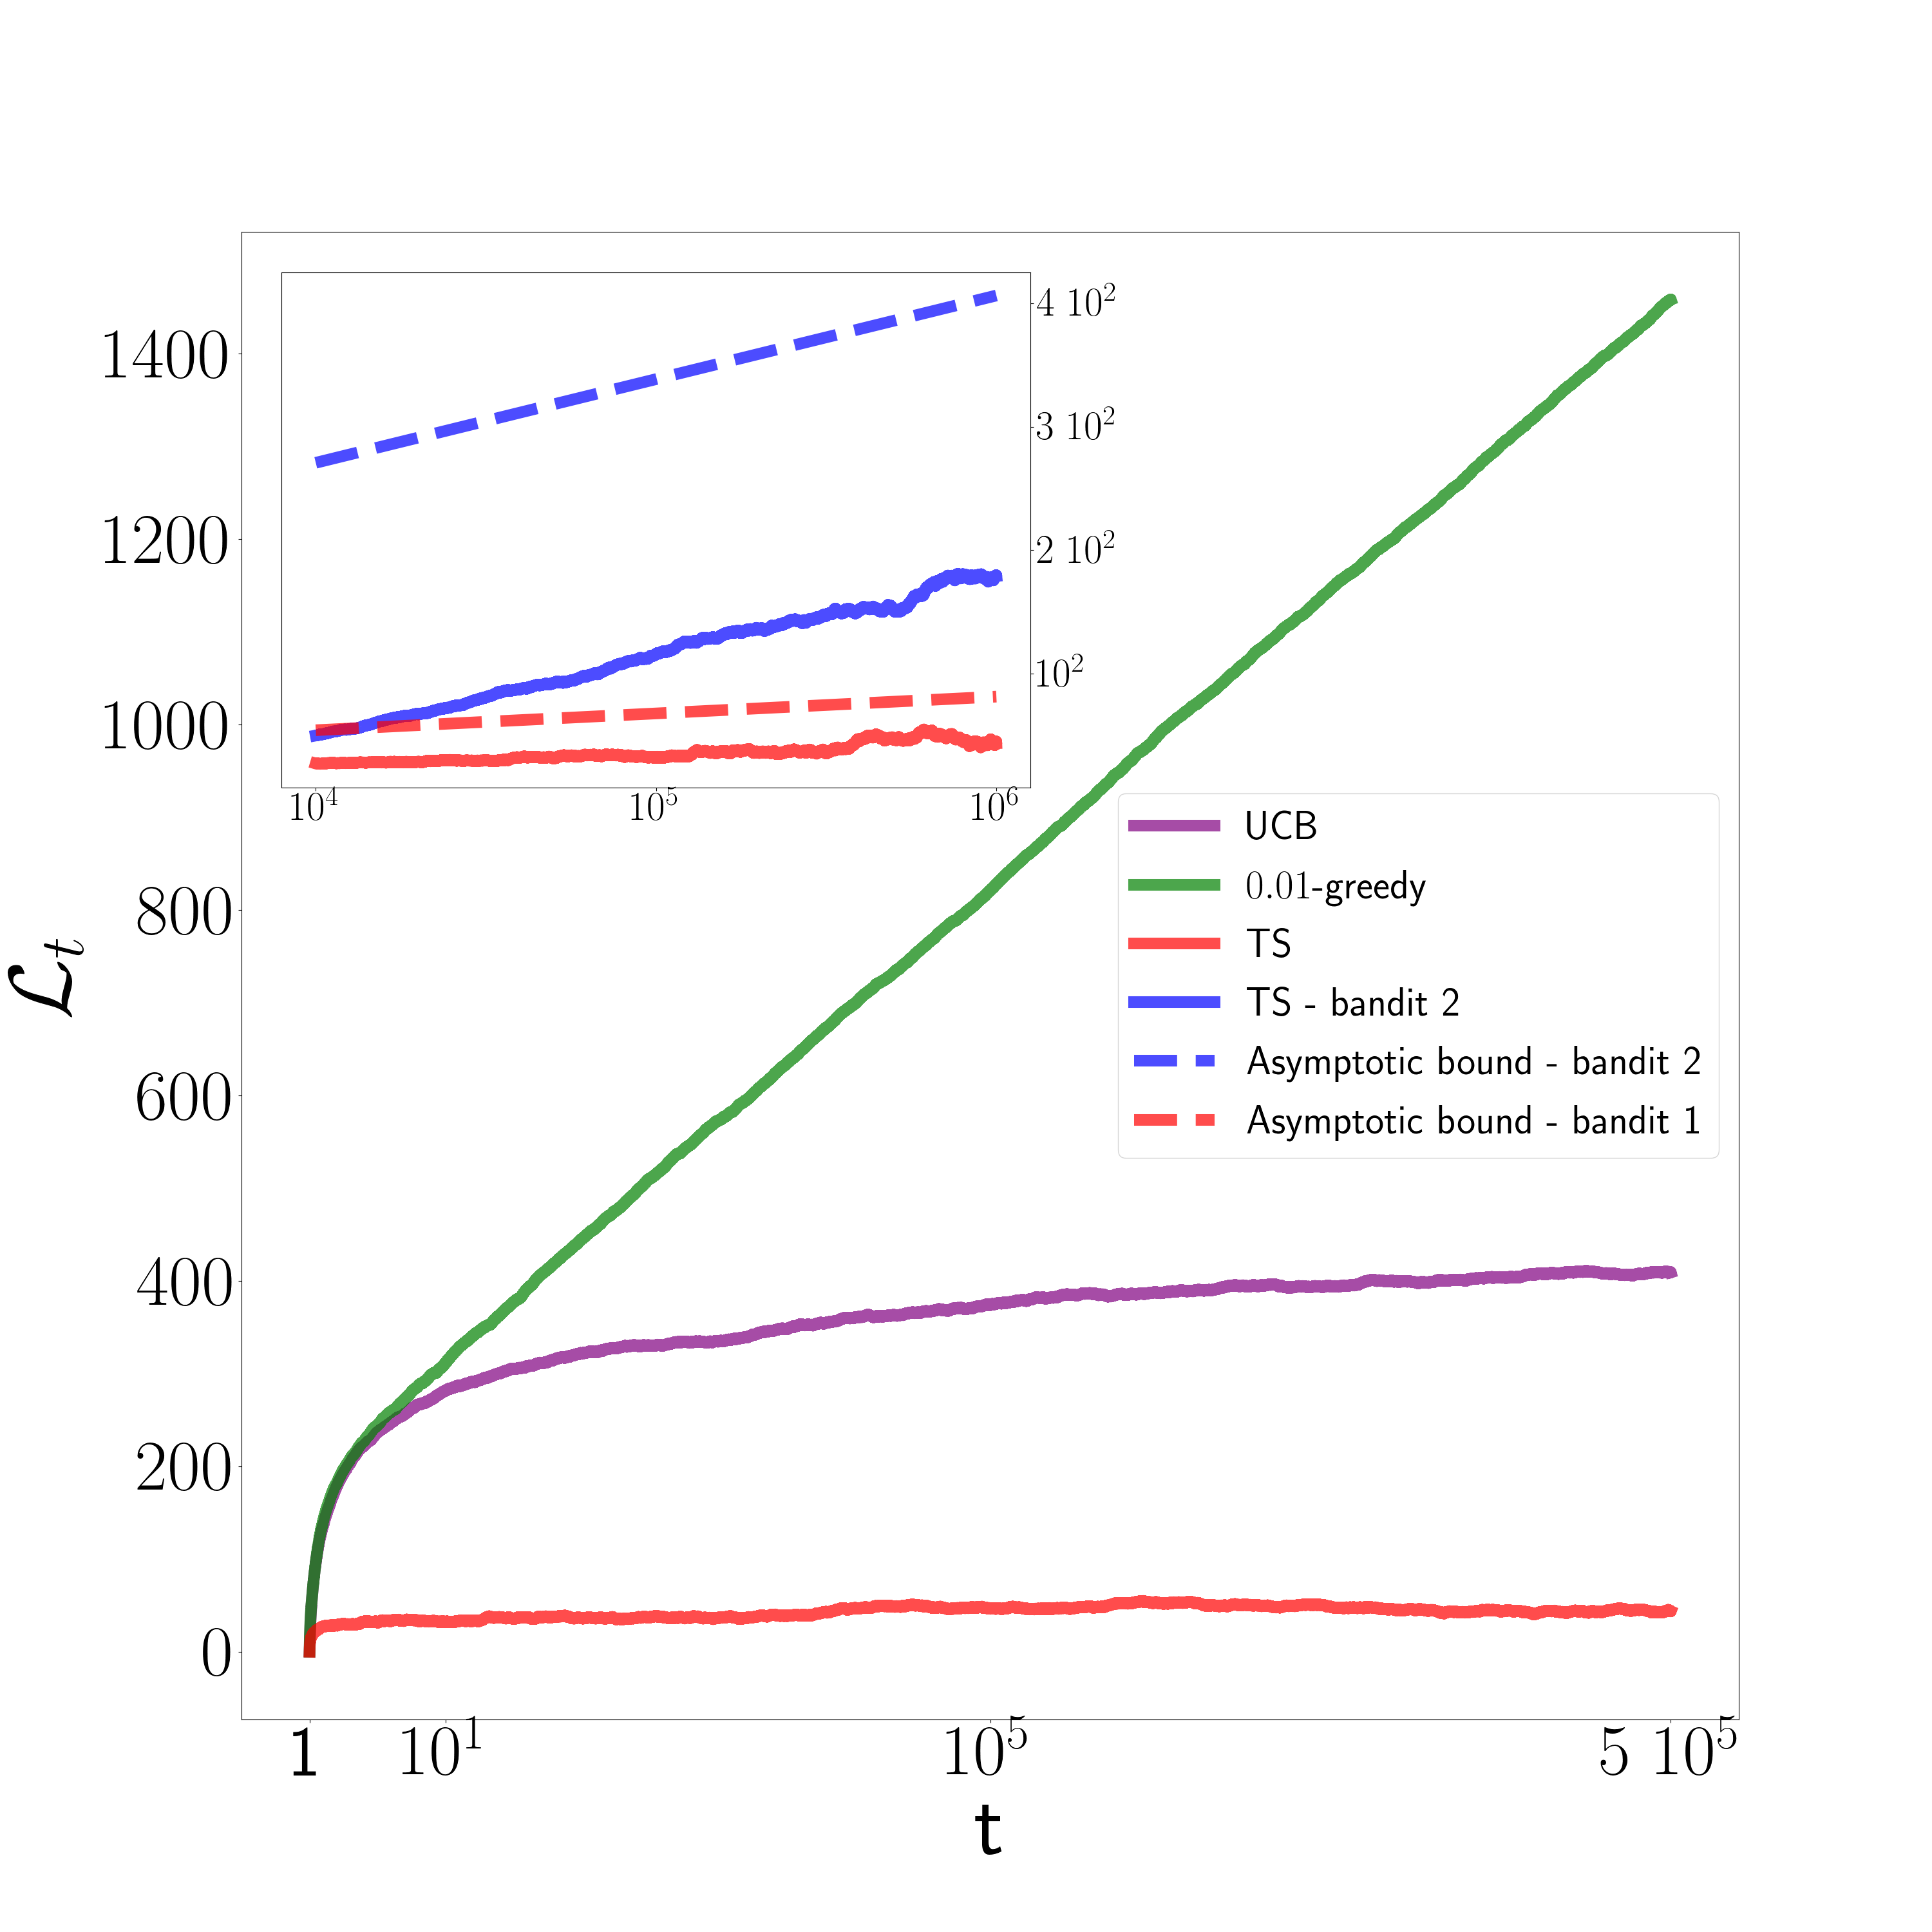
\includegraphics[width=0.8\textwidth]{Figures/1bandit/bandit_numerics_not_shifted.png}
    \caption{We show the evolution of the cumulative regret for three different policies: $\varepsilon$-greedy, UCB and TS in a bandit setting. The mean values considered are associated to success probabilities of Kennedy-like receivers, which we will introduce in Sec.~\ref{ssec:rlcoh_kennedyreceiver}.  All curves are averaged  over $10^{3}$ agents. Specifically, they are Bernoulli distributions with different mean values, each associated to different configurations of a quantum receiver parametrized by a value $\beta$. For \textit{bandit problem 1}, we considered $\beta \in \{0, -\alpha, \beta^{*}\}$, with $\alpha = 0.4$ and $\beta^{*} = -0.74$.
    Furthermore, we compare the asymptotic behaviour of TS, studying \textit{bandit problem 2}, where $\beta \in \{-\alpha, \beta^{*}, -1.5 \alpha\}$, shown in the inset plot.}
    \label{fig:bandfig}
\end{figure}

To complement this section on the bandit problem, we have numerically compared the performance of the three policies introduced above. In Fig~\ref{fig:bandfig} we show the expected regret $\mathcal{L}_t$ estimated out of several realizations of a 3-armed bandit problem. The distributions considered are Bernoulli distributions with different mean values; at each episode the agent observes a reward of value either $0$ or $1$, drawn from the corresponding Bernoulli distribution. The figure shows that the cumulative regret scales linearly with time for the $\epsilon$-greedy strategy, while it has a logarithmic scaling for the UCB and TS strategies. The inset shows the cumulative regret as a function of $\log t$ together with the ultimate bound given by Lai-Robbins bound; we observe that sub-leading constants seem to still be relevant in such a bound, and that whereas assymptotic regime seems not to have been reached, the results are yet consistent with Eq.~\ref{eq:RLBOUND}. Moreover, the distributions we have considered are linked to success probabilities of different configurations of a quantum receiver,
called Kennedy-like receiver, which we introduce in Sec.~\ref{ssec:rlcoh_kennedyreceiver}.

Let us conclude this overview of bandit theory by introducing the \textit{simple regret}, another widely used figure of merit that quantifies how well has the agent learned to identify the optimal action at episode $t$, regardless of her actual performance:
\begin{equation}
\Lambda_t = \mathbb{E} \big(Q(a^{*}) - Q(a^{(t)*}) \big),
\end{equation}
where $a^{(t)*}$ is the agent's \emph{recommendation} of which the optimal action is at episode $t$. For example, in an $\epsilon$-greedy strategy, the recommendation is given by $a^{(t)*}=argmax_{a}\hat{Q}(a)$. Thus, strategies designed to minimize $\Lambda_t$ will prioritize to learn what the optimal arm to pull is, regardless of the rewards acquired during the entire learning process.%, and the probability that the agent confuses the optimal arm by a sub-optimal one will be exponentially small, hence $\Lambda_t $ will converge to zero exponentially fast.
Recent results~\cite{simpleRegretMunoz} show that the exploitation-exploration trade-off manifests itself in the asymptotic scaling of the simple and cumulative regret in the sense that one imposes lower and upper-bounds on the other, and therefore optimizing one usually affects the performance of the other.

Having gained some intuition on why model-free learning schemes are complex, we will not return to study the general MDP setting.
